%!TEX root = ../../main.tex

\subsubsection{AI Pathfinding}
The ghost AI of the original Pac-Man is based on a single pathfinding algorithm which all the modes previously discussed in the investigation utilize \cite{Pittman2011}.
In order to get a better understanding of how these modes work we need to look at this pathfinding mechanism.

The maze is made up of tiles in a grid.
This grid has a size of 28 x 36 tiles, this includes everything on the screen including score counters, and life count.
The size of the individual tiles depends on the resolution of the game space.
In the case of the origin Pac-Man the screen size was 224 x 288 pixels.
That makes each tile 8 x 8 pixels in size.

The pathfinding works by finding a path from one tile to the other using only the tiles that are walkable within the maze.
Tiles outside the maze and tiles with pieces of wall within them, while still tiles in the collection of tiles, are considered illegal tiles.

\begin{figure}[!htbp]
\centering
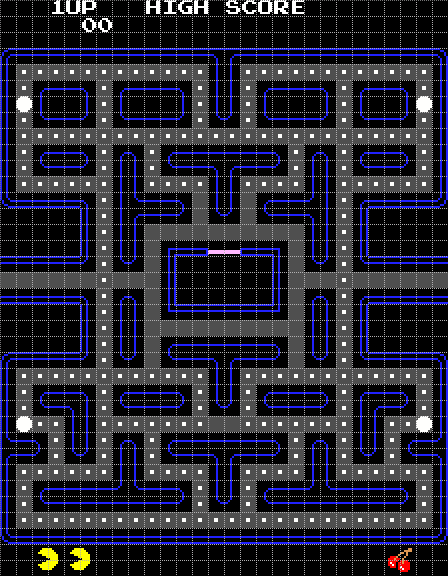
\includegraphics[width=0.5\textwidth]{Tiles.png}
\caption{Visible space in a game of Pac-Man: \cite{Pittman2011} }
\label{fig:Pacman_visible_space}
\end{figure}

While the ghosts can only move along a path using legal tiles, their target tile can be anywhere on the grid.
In chase mode the target tile will be somewhere near the Pac-Man (depending on the ghost in question), and in scatter mode where the ghost will move towards its designated corner of the maze.
The target tile the ghost will go to when in scatter mode is fixed outside of the maze to ensure that the ghost will never get to it, resulting in the ghost circulating in the area closest to the fixed target until it has a new target.
Another fixed tile is the one in the ghost-one in the middle of the screen.
This is activated when the ghost has been eaten by the Pac-Man and is sent back to the pen.

In Figure \ref{fig:Pacman_visible_space} we can see the grid laid out over the screen of Pac-Man. The grey tiles are considered walkable and the tiles that the pathfinding works with. The eatable pellets are the white dots in the middle of those tiles.

The bulk of the pathfinding happens when the ghost reaches an intersection in the maze.
When the ghost is one tile away from an intersection, it will adjust its direction.
It works by finding the tile with the shortest distance to the target.
It looks one ahead in every direction of the intersection and chooses whichever direction has the shortest distance to the target.
When a ghost is presented with a tie, meaning an intersection where two or more directions have equal distance to the target, the ghost will default to choosing the direction in a specific order: \emph{up, left, down, right}\cite{Pittman2011}.
This means that when the ghost is in a tie situation it will always choose the an upwards direction before left, if those two were the tie directions.
